\documentclass[onecolumn,10pt]{jhwhw}

\usepackage{epsfig} %% for loading postscript figures
\usepackage{amsmath}
\usepackage{graphicx}
\usepackage{grffile}
\usepackage{pdfpages}
\usepackage{algpseudocode}
\usepackage{wrapfig}
\usepackage{pgfplots}
\usepackage{amsfonts}
\usepackage{booktabs}
\usepackage{siunitx}
\usepackage{commath}
\usepackage{rotating}
\usepackage{url}
\usepackage{multimedia}
\usepackage{hyperref}
\usepackage{mathtools}

% Default fixed font does not support bold face
\DeclareFixedFont{\ttb}{T1}{txtt}{bx}{n}{12} % for bold
\DeclareFixedFont{\ttm}{T1}{txtt}{m}{n}{12}  % for normal

% Custom colors
\usepackage{color}
\usepackage{listings}
\usepackage{framed}
\usepackage{caption}
\usepackage{bm}
\captionsetup[lstlisting]{font={small,tt}}

\definecolor{mygreen}{rgb}{0,0.6,0}
\definecolor{mygray}{rgb}{0.5,0.5,0.5}
\definecolor{mymauve}{rgb}{0.58,0,0.82}

\lstset{ %
  backgroundcolor=\color{white},   % choose the background color; you must add \usepackage{color} or \usepackage{xcolor}
  basicstyle=\ttfamily\footnotesize, % the size of the fonts that are used for the code
  breakatwhitespace=false,         % sets if automatic breaks should only happen at whitespace
  breaklines=true,                 % sets automatic line breaking
  captionpos=b,                    % sets the caption-position to bottom
  commentstyle=\color{mygreen},    % comment style
  deletekeywords={...},            % if you want to delete keywords from the given language
  escapeinside={\%*}{*)},          % if you want to add LaTeX within your code
  extendedchars=true,              % lets you use non-ASCII characters; for 8-bits encodings only, does not work with UTF-8
  frame=single,                    % adds a frame around the code
  keepspaces=true,                 % keeps spaces in text, useful for keeping indentation of code (possibly needs columns=flexible)
  columns=flexible,
  keywordstyle=\color{blue},       % keyword style
  language=Python,                 % the language of the code
  morekeywords={*,...},            % if you want to add more keywords to the set
  numbers=left,                    % where to put the line-numbers; possible values are (none, left, right)
  numbersep=5pt,                   % how far the line-numbers are from the code
  numberstyle=\tiny\color{mygray}, % the style that is used for the line-numbers
  rulecolor=\color{black},         % if not set, the frame-color may be changed on line-breaks within not-black text (e.g. comments (green here))
  showspaces=false,                % show spaces everywhere adding particular underscores; it overrides 'showstringspaces'
  showstringspaces=false,          % underline spaces within strings only
  showtabs=false,                  % show tabs within strings adding particular underscores
  stepnumber=1,                    % the step between two line-numbers. If it's 1, each line will be numbered
  stringstyle=\color{mymauve},     % string literal style
  tabsize=4,                       % sets default tabsize to 2 spaces
}

\usepackage{etoolbox}
\renewcommand{\lstlistingname}{Diagram}% Listing -> Algorithm
\patchcmd{\thebibliography}{\chapter*}{\section*}{}{}

\author{John Karasinski}
\title{Homework 3}

\begin{document}
%\maketitle

\problem{Develop a very simple representation of the Hubble telescope.}
\begin{lstlisting}[caption={Hubble ASCII Diagram. Solar panel distance from HST is exaggerated. One character is $\approx$ 20 inches.}]
#########################################################################################
#                                         Hubble                                        #
#     ^V2                                                                               #
#     |                          +----------------------+                               #
#  <--+                          |                      |                               #
#  V1                            |         SA1          |                               #
#                                |                      |                               #
#                                +-----------+----------+                               #
#                                            |                                          #
#                                            |    +-------+                             #
#                             +--------------++---+       |                             #
#                             |               |   |       |                             #
#                             |       1       | 2 |   3   |                             #
#                             |               |   |       |                             #
#                             |               |   |       |                             #
#                             +--------------++---+       |                             #
#                                            |    +-------+                             #
#                                            |                                          #
#                                +-----------+----------+                               #
#                                |                      |                               #
#                                |         SA1          |                               #
#                                |                      |                               #
#                                +----------------------+                               #
#                                                                                       #
#########################################################################################
#                                                                                       #
#     ^V3                                                                               #
#     |                                                                                 #
#  <--+                                           +-------+                             #
#  V1                         +---------------+---+       |                             #
#                             |               |   |       |                             #
#                             |       1       | 2 |   3   |                             #
#                             |  +-----------+----------+ |                             #
#                             |               |   |       |                             #
#                             +---------------+---+       |                             #
#                                                 +-------+                             #
#                                                                                       #
#                                                                                       #
#                                                                                       #
#########################################################################################
\end{lstlisting}
% #                                                                                       #
% #     ^V3                                                                               #
% #     |                                                                                 #
% #  <--+                         +---+                  +---+                            #
% #  V2                           |   |                  |   |                            #
% #                               |   |     ________     |   |                            #
% #                               |   |    /  *--*  \    |   |                            #
% #                               |   |   / *      * \   |   |                            #
% #                               |   +--| *        * |--+   |                            #
% #                               |   |   \ *      * /   |   |                            #
% #                               |   |    \  *--*  /    |   |                            #
% #                               |   |      ------      |   |                            #
% #                               |   |                  |   |                            #
% #                               +---+                  +---+                            #
% #                                                                                       #
% #                                                                                       #
% #########################################################################################

\begin{figure}[tbh!]
\begin{center}
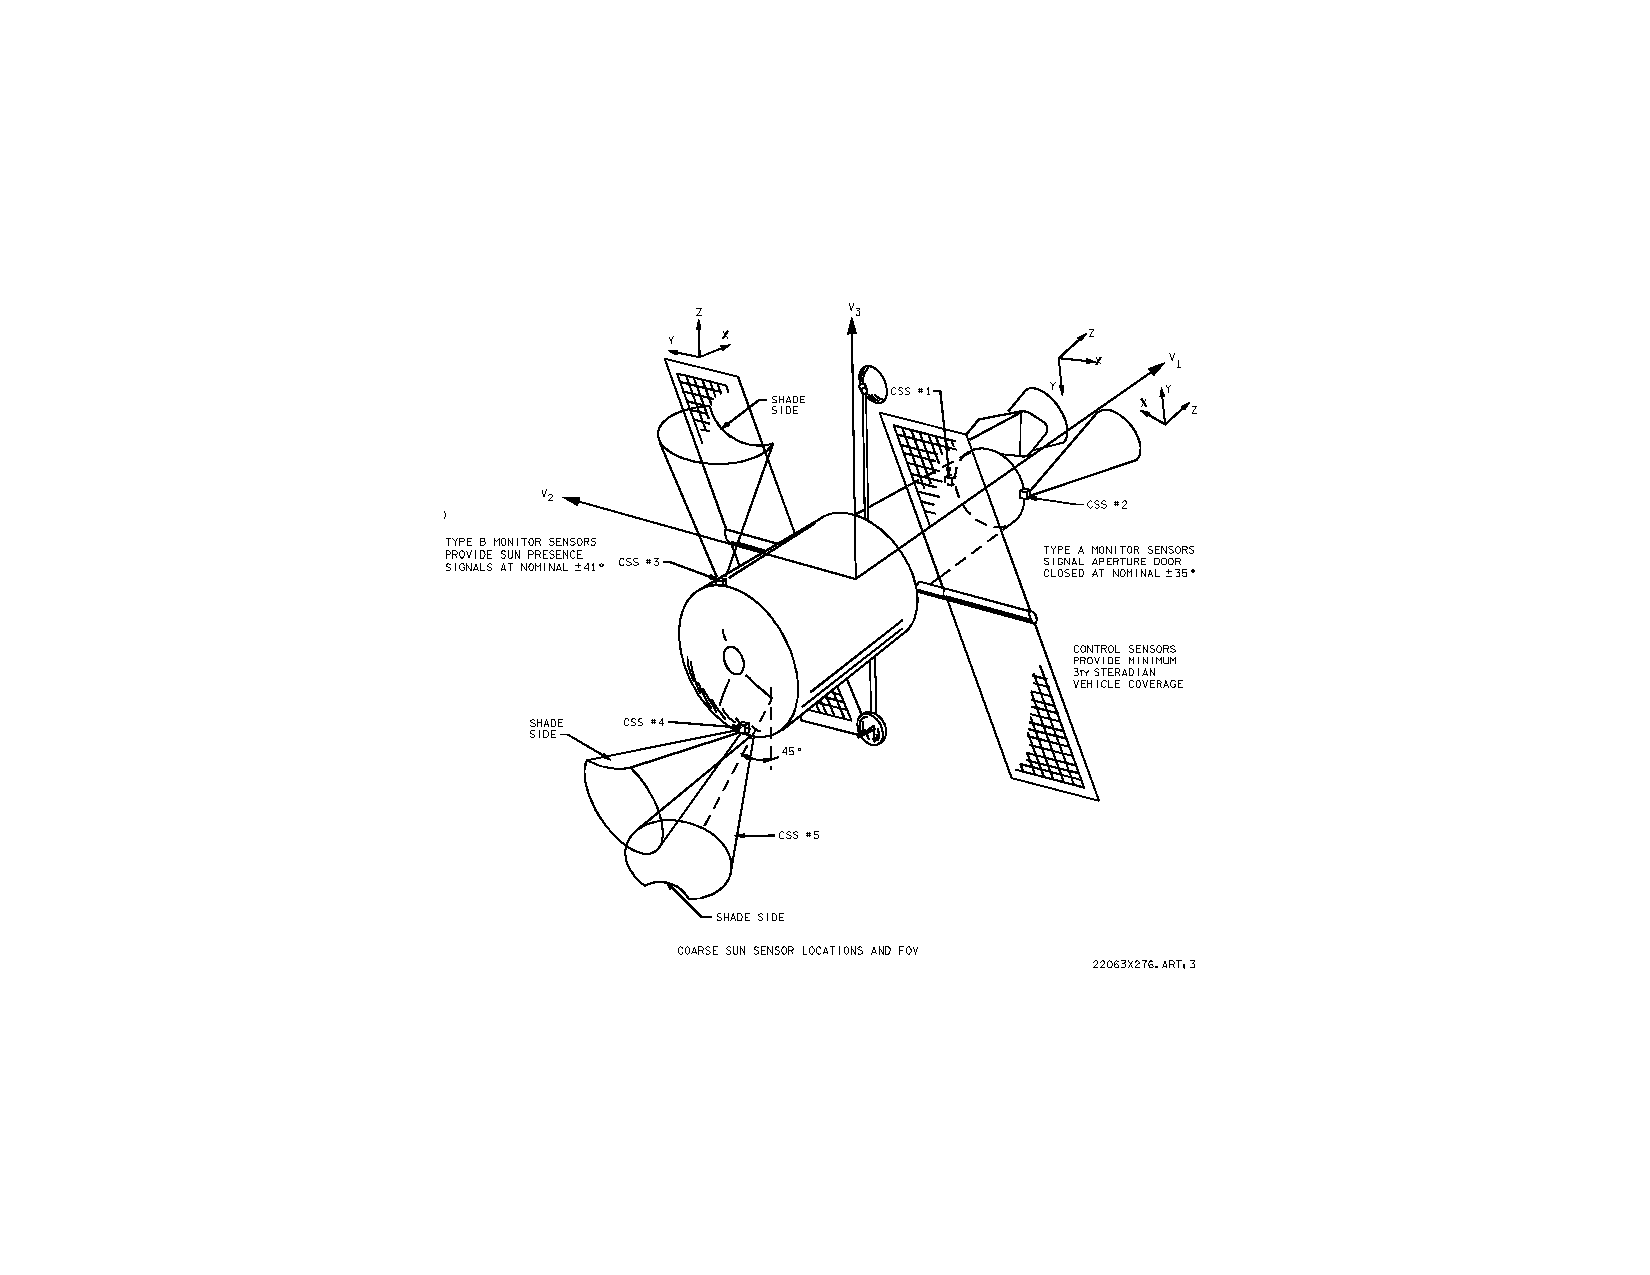
\includegraphics[height=0.4\textheight]{hst_axes.pdf}
\label{fig:on}
\end{center}
\caption{HST Axes Definition for $V_1, V_2, V_3$, CG is located at axis origin}
\end{figure}

We model both the body (3 sections) and the solar panels (2 sections) of the Hubble Space Telescope (HST). The body sections are connected as such: Section 1 is connected to Section 2, and Section 2 is connected to Section 3. The solar arrays are connected on Section 1, along the centerline, 20.75 inches $V_1$ away from the connection point with Section 2, and the near edge of the SA is 129 inches from center of Section 1. These sections are modeled with thin walled cylinders (TWC), solid cylinders (SC), and flat plates (FP). The rough layout of the sections is shown on the previous page, and the mass and length properties of each section are listed in Table~\ref{properties}.

\begin{table}[t!]
\begin{center}
\begin{tabular}{l r r r r r}
\toprule
Section & Model & $V_1$ (in) & $V_2$ (in) & Weight (lb) \\
\midrule
\it{Section 1} & & & & \\
\hspace{1em} Light Shield (LS)   & - & 153.2  & 120  & - \\
\hspace{1em} Forward Shell (FS) (except OTA)  & - & 156.05 & 121.2 & - \\
\hspace{1em} Total  & TWC & 270.75 & 121.2 & 2796 \\
\it{Section 2} & & & & \\
\hspace{1em} OTA Equipment Section  & TWC & 38.5 & 121.2 & 9033 \\
\it{Section 3} & & & & \\
\hspace{1em} SSM Equipment Section (SSM-ES) & - &  61.25  &  168.16 & 10594\\
\hspace{1em} Aft Shroud (AS) & - &  138.00  &  168.16 & 569\\
\hspace{1em} Total  & SC & 199.25 & 168.16 & 11163 \\
\it{Section 4} & & & & \\
\hspace{1em} Solar Arrays (SA) & FP &  476.8$^1$  &  113.5 & 735$^2$\\
\bottomrule
\end{tabular}
\end{center}
\caption{$^1$: This length can be fully rotated into $V_3$. $^2$: Weight of both solar arrays. $V_1$ and $V_2$ indicate the measurements of the parts. All lengths taken from Hubble technical drawings~\cite{hst}; all masses from~\cite{mil}.}
\label{properties}
\end{table}

\problem{Use this model as a basis to write a function(s) to determine the Mass Center and Inertia Matrix for any location.}

Using the radial-center of the farthest tip of Section 1 as our zero point , the center of mass is located at $V = [327, 0, 0]$ inches. This makes since, as the model is symmetric about the $V_2$ and $V_3$ axes, and this value is on the boundary between Section 2 and Section 3, which is very close to where the reaction wheels are located.

The HST inertia matrix~\cite{HRV}, was at one point measured as:
\begin{align*}
I =
\begin{bmatrix*}[r]
    36046       & -706  &  1491 \\
    -706        & 86868 &   449 \\
    1491        & 449   & 93848
\end{bmatrix*}
kg \cdot m^2.
\end{align*}
The Python script in Appendix gives the result of:
\begin{align*}
I =
\begin{bmatrix*}[r]
   35914 &      0 &      0 \\
       0 & 88215 &      0 \\
       0 &      0 & 113393
\end{bmatrix*}
kg \cdot m^2,
\end{align*}
which has a relative error of:
\begin{align*}
I =
\begin{bmatrix*}[r]
  0 & 100 & 100 \\
100 &  -2 & 100 \\
100 & 100 & -21
\end{bmatrix*}
\%.
\end{align*}
Note that while our simple, 5 part model does a very good job of predicting the $I_{V_1}$ and $I_{V_2}$ components, the $I_{V_3}$ component is not represented very well. This is likely due to leaving out the antenna booms, which should have the largest effect in the $V_3$ directions. It should also be noted that, due to the symmetric nature of our model, all of the off-axis terms are missing. For the rest of the analysis, the true values for the inertia matrix will be used. See Figure~\ref{fig:inert} for the effects of rotating the solar arrays on the principle axes.

\begin{figure}[h!]
\begin{center}
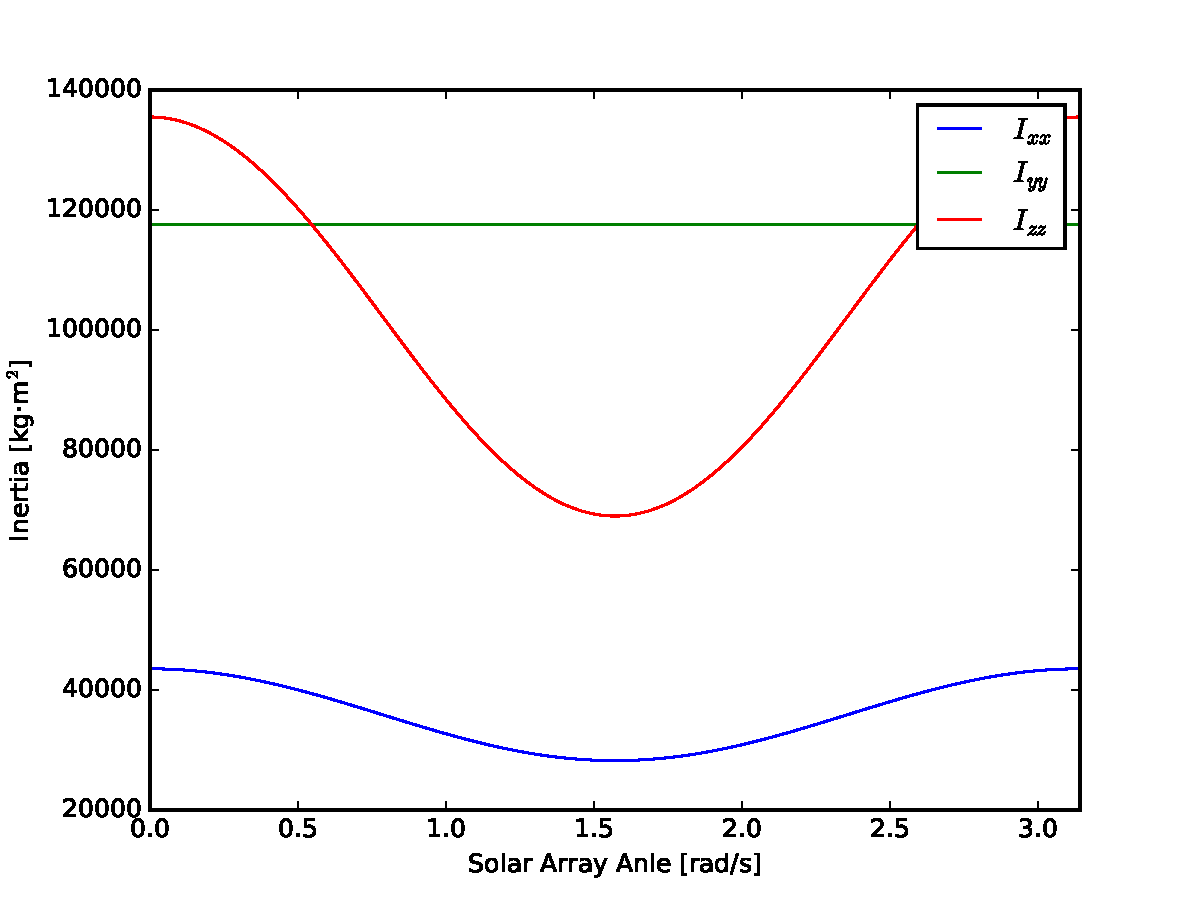
\includegraphics[height=0.41\textheight]{figure1.pdf}
\end{center}
\caption{Inertias for principal axes for different solar array configurations}
\label{fig:inert}
\end{figure}

\problem{Write a function to find the current angular momentum relative to the mass center.}

$H$ increases linearly with $\omega$. See Appendix for the code used to create Figure~\ref{fig:spin}.

\begin{figure}[h!]
\begin{center}
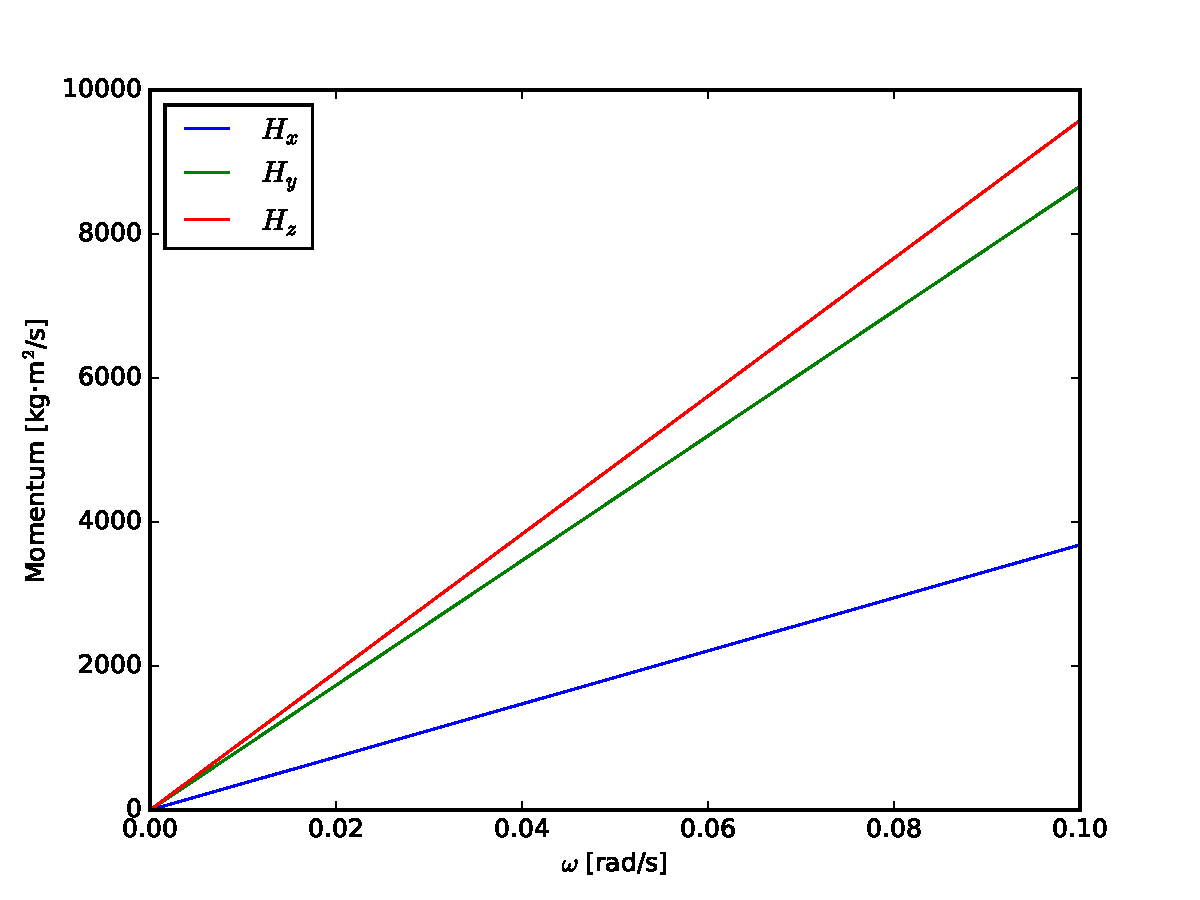
\includegraphics[height=0.41\textheight]{figure2.pdf}
\end{center}
\caption{Effects of spin on each axis}
\label{fig:spin}
\end{figure}

\problem{Choose the optimal location for a torque producing system and explain why you think is the best location.}

\begin{figure}[h!]
\begin{center}
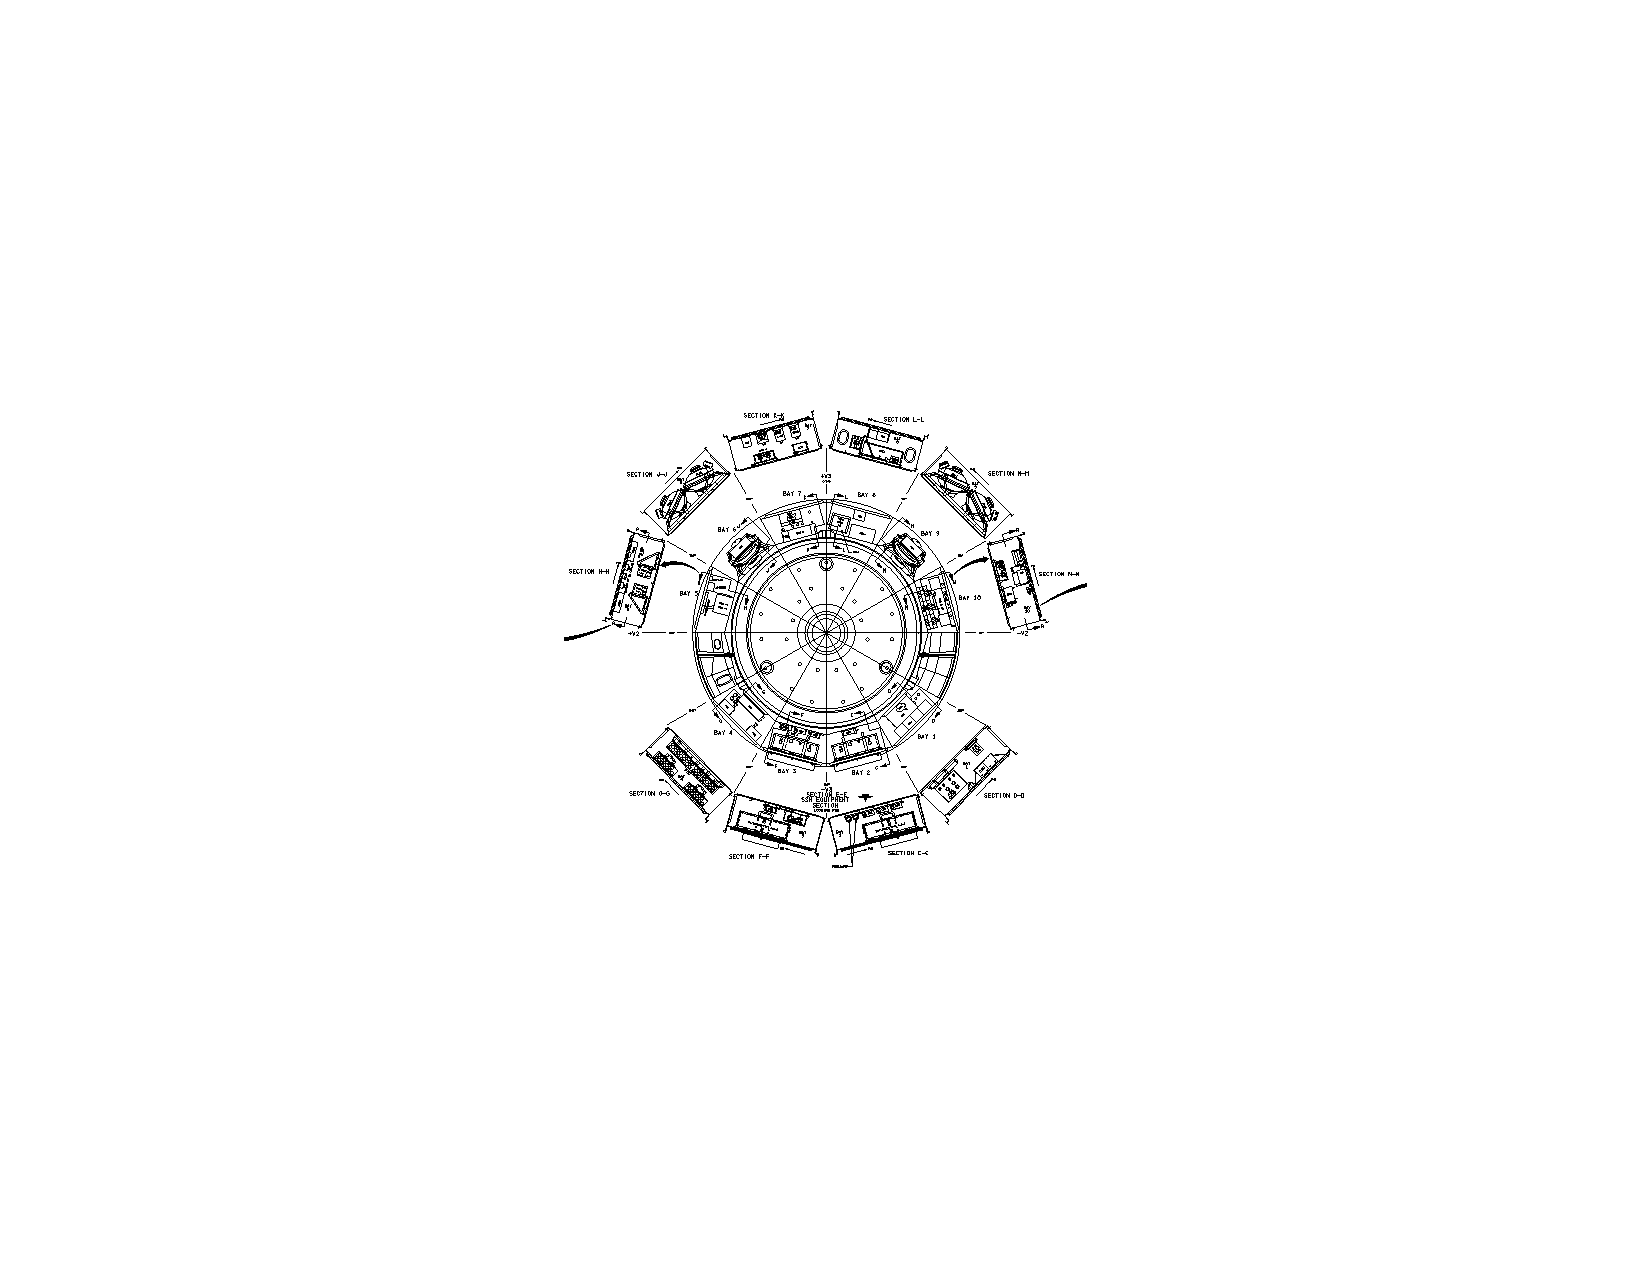
\includegraphics[height=0.5\textheight]{hst_rw.pdf}
\end{center}
\caption{HST's reaction wheels are located in the SSM-ES in bays 6 and 9. The pairs were installed in at a 90$^o$ offset to protect against failures~\cite{hst}.}
\label{fig:rw}
\end{figure}

The optimal location for a torque producing system is usually on the centerline, as near to the center of mass of the spacecraft as possible. Placing the torque producing system close the the spacecraft's center of mass minimizes the amount of undesirable resultant torque when the system is activated. In HST's case, the optimal location for a torque producing system is in the SSM-ES, see Fig.~\ref{fig:rw}. The two wheels of a single SSM bay are canted off the $V_2$-$V_3$ plane by 20$^o$, one toward the +$V_1$ and one toward the -$V_1$. I think that this is likely the best location to place the system as it's the one that was actually used, and because the engineers that placed them the reaction wheels there had much greater access to information about HST than I do.

As we do not have to worry about reaction wheels failing for the purposes of this homework, I would instead simplify the system to a single location of three reaction wheels, one of which is aligned with each axis. ``Nominal dynamic torque range is 0.003 to 0.605 ft-lb (0.004 to 0.7 N$\cdot$m), with a maximum wheel speed of $\pm$3000 rpm'' for each of the four reaction wheels~\cite{hst}.

\problem{Using your previous functions, write a program to find the resulting angular acceleration produced from a given torque.}

\begin{figure}[h!]
\begin{center}
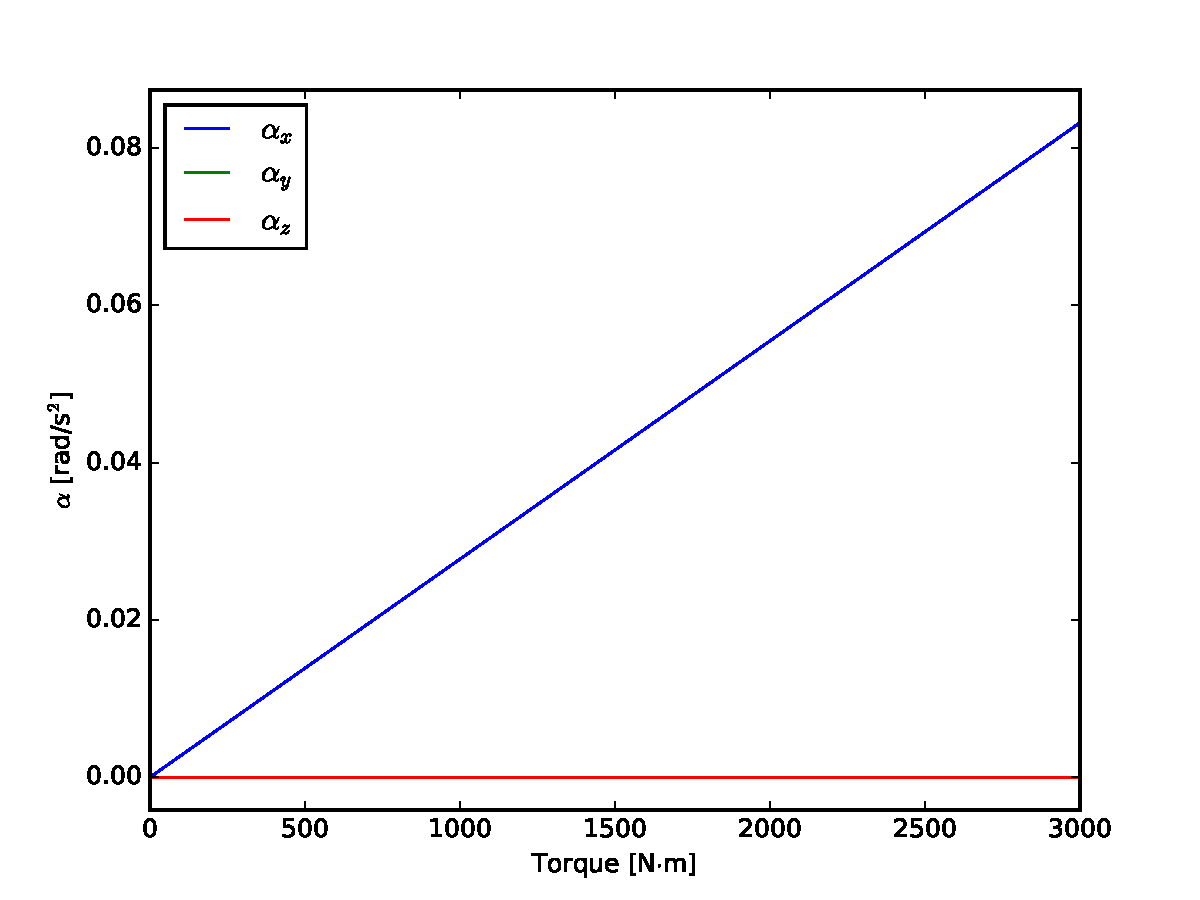
\includegraphics[height=0.4\textheight]{figure3.pdf}
\label{fig:on}
\end{center}
\caption{Angular acceleration response along all three axis from a single reaction wheel producing $\tau_x$, from initial conditions $\omega = [0, 0, 0]$ rad/s.}
\end{figure}

\begin{figure}[h!]
\begin{center}
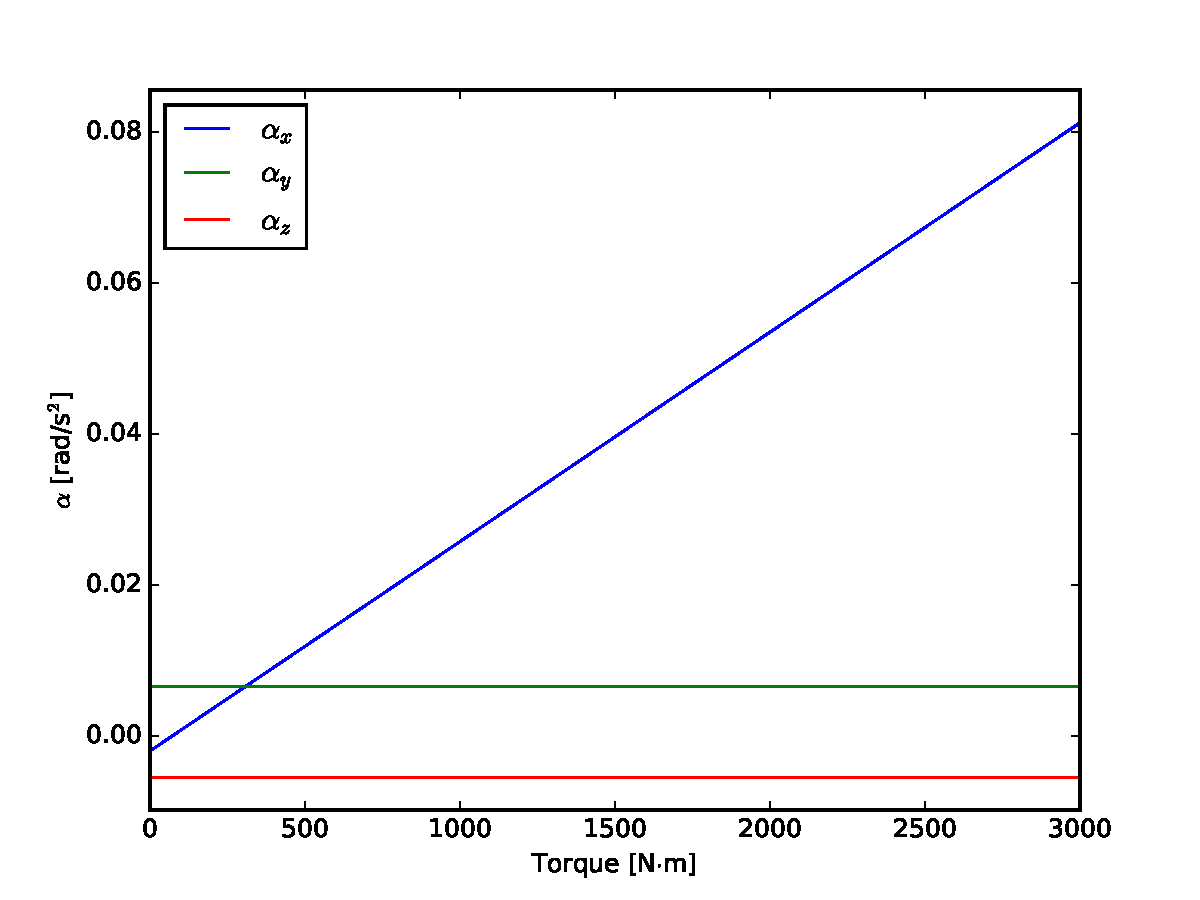
\includegraphics[height=0.4\textheight]{figure4.pdf}
\label{fig:on}
\end{center}
\caption{Angular acceleration response along all three axis from a single reaction wheel producing $\tau_x$, from initial conditions $\omega = [0.1, 0.1, 0.1]$ rad/s.}
\end{figure}

\clearpage
\problem{Write what next steps you would take to develop a controller that keeps the craft pointed in a specific direction.}

To develop a controller, we would need to:
\begin{enumerate}
\item Determine where the craft should be pointed (science requirements)
\item Determine where the craft is currently pointed (using sensors)
\item Find the difference between these two (the error)
\item Determine which reaction wheels need to be activated to minimize the error
\item Activate the reaction wheels
\end{enumerate}

Once we had sensors and the ability to activate our reaction wheels, the majority of the time developing the controller would involve tuning it to perform to some specification (minimizing overshoot, minimizing response time, etc.).

\bibliographystyle{IEEEtran}
\begin{thebibliography}{1}
\bibitem{HRV}
Queen, S., ``HRV GNC Peer Review, Flight Performance Analysis,'' Tech. rep., NASA Goddard Space Flight Center, 2004.

\bibitem{hst}
NASA, ``Cargo Systems Manual (CSM): Hubble Space Telescope,'' February 13, 2002

\bibitem{mil}
Mattice, J., ``Hubble Space Telescope Systems Engineering Case Study.''
\end{thebibliography}

\appendix
\section{Python Code}
\lstinputlisting{hw3.py}

\end{document}
